\documentclass[bibliography=totoc]{scrartcl}
\usepackage{diagbox}
\usepackage{color}
\definecolor{indianred}{rgb}{0.8, 0.36, 0.36}
\definecolor{dodgerblue}{rgb}{0.12, 0.56, 1.0}
\usepackage{scrhack}
\usepackage[a4paper,top=2.5cm,right=2.5cm,left=2cm,bottom=3cm,bindingoffset=5mm]{geometry}
\usepackage[aux]{rerunfilecheck}
\usepackage{fontspec}
% \setmainfont{Cambria}
\usepackage{polyglossia}
\setmainlanguage{german}

\usepackage[
  %style = numeric,
  %natbib = true,
  sorting = none
]{biblatex}
\addbibresource{lit.bib}

\usepackage{amsmath}
\usepackage{amssymb}
\usepackage{mathtools}

\newcolumntype{P}[1]{>{\centering\arraybackslash}p{#1}}

\usepackage[
  math-style=ISO,
  bold-style=ISO,
  sans-style=italic,
  nabla=upright,
  partial=upright,
]{unicode-math}

\usepackage[
  locale=DE,
  separate-uncertainty=true,
  per-mode=symbol-or-fraction,
]{siunitx}
\sisetup{exponent-product = \cdot, output-decimal-marker = {,}, per-mode = fraction}
\DeclareSIUnit\atm{atm}
%\usepackage[section]{placeins}
\usepackage{subcaption}
\usepackage{float}
\usepackage{xcolor}
\definecolor{tugrun}{RGB}{133,184,21}
\usepackage{sectsty}
\chapterfont{\color{tugrun}}
\sectionfont{\color{tugrun}}
\subsectionfont{\color{tugrun}}
\subsubsectionfont{\color{tugrun}}
\usepackage{tocloft}
\renewcommand\cftsecfont{\color{tugrun}}
\renewcommand{\cfttoctitlefont}{\color{tugrun}\Large\bfseries}

\usepackage{fancyhdr}
\pagestyle{fancy}
\renewcommand{\sectionmark}[1]{\markright{#1}}
\renewcommand{\subsectionmark}[1]{}
\usepackage{etoolbox}
\patchcmd{\headrule}{\hrule}{\color{tugrun}\hrule}{}{}
% \lhead{Versuch B14: Tomographie mittels $\gamma$-Strahlung}
\lhead{\rightmark}
\rhead{\texorpdfstring{\href{mailto:felix.landmeyer@tu-dortmund.de}{Felix Landmeyer} \\
\texorpdfstring{\href{mailto:melina.helfrich@tu-dortmund.de}{Melina Helfrich}}}}
\renewcommand{\headrulewidth}{2pt}


% \usepackage[headsepline,automark]{scrlayer-scrpage}
% \clearpairofpagestyles
% \ihead{\rightmark}
% \ofoot{\pagemark}
% \addtokomafont{pageheadfoot}{}
%
% \KOMAoptions{onpsinit=\setstretch{1}}
% \renewcommand*\chaptermarkformat{}
% \renewcommand*\chapterpagestyle{scrheadings}



\restylefloat{table}
\floatplacement{figure}{htbp}
\floatplacement{table}{t}
\floatstyle{plaintop}
\restylefloat{table}

\usepackage[
version=4,
math-greek=default,
text-greek=default,
arrows=pgf,
]{mhchem}


\usepackage[unicode]{hyperref}
\usepackage{bookmark}
\usepackage{microtype}
\usepackage{multirow}
\usepackage[section]{placeins}
\usepackage{caption}
\usepackage{eso-pic}
\usepackage{graphicx}
\usepackage{grffile}
\usepackage{microtype}
\usepackage{xfrac}
\usepackage{wrapfig}
\usepackage{tkz-euclide}
\usetkzobj{all}
\usepackage{array}
\usepackage{booktabs}
\usepackage{icomma}
\setkomafont{captionlabel}{\normalsize\bfseries}
\setkomafont{sectioning}{\bfseries}
\setlength\parindent{0pt}
\usepackage{cancel}
\begin{document}
\begin{titlepage}
  \centering
  
\includegraphics[width=0.5\textwidth]{content/Logo.jpg}\par\vspace{2cm}
  {\scshape\LARGE Technische Universität Dortmund \par}
  \vspace{1.5cm}
  {\scshape\Large Fortgeschrittenen Praktikum \par}
  \vspace{1.5cm}
  {\scshape\LARGE\bfseries V27 Zeeman-Effekt\par}
  \vspace{2.5cm}
  {\Large Melina Helfrich, \texorpdfstring{\href{mailto:melina.helfrich@tu-dortmund.de}{melina.helfrich@tu-dortmund.de}}\par\par
  \par\vspace{0.25cm}
  Felix Landmeyer, \texorpdfstring{\href{mailto:felix.landmeyer@tu-dortmund.de}{felix.landmeyer@tu-dortmund.de}}\par\par}
  \vspace{2cm}
  {\scshape Durchführung am 13.01.2020 \par
    Abgabe am  \par
    %Korrekturabgabe am ..2020
    }
\end{titlepage}
%\newpage
%\tableofcontents
%\newpage
%\setcounter{page}{3}
\section{Theoretische Grundlagen}
Ziel dieses versuches ist es mithilfe des Faraday-Effektes die effektive Masse der Leitungselektronen in 
Galium-Arsenit zu bestimmen. \\
\\
Der Faraday-Effekt, der auch als Faraday-Rotation bezeichnet wird, beschreibt die Drehung der
Polarisationsrichtung einer linear polarisierten Welle bei dem Durchgang durch ein Medium 
unter dem Einfluss eines äußeren Magnetfeldes. Mithilfe dieses Effektes ist es möglich die 
Bandstruktur unterschiedlicher Materialien zu verstehen. \\

\subsection{Beschreibung der Bandstruktur}
Wenn über die Bandstruktur gesprochen wird, ist die Rede von einem Valenz- und einem Leiterband. 
Dabei entspricht das Valenzband dem höchsten besetzten Energieband. Das Energieband, das sich über dem 
Valenzband befindet, wird als Leiterband bezeichnet. \\
Diese Energiebänder entstehen aufgrund hinreichend großer Annäherung von Atomen. Dadurch kommt es zum 
Überlappen der Atomorbitale und durch die Superposition dieser zur Entstehung der Energiebänder. \\
Anhand der Energiebänder ist es möglich Materialien in Isolatoren, Halbleiter und Metalle zu unterteilen. 
In Abbildung \ref{fig:Bandstrukturen} sind die unterschiedlichen Bandstrukturen schematisch abgebildet.
\begin{figure}[H]
    \centering
    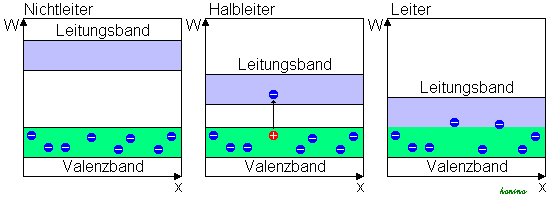
\includegraphics[width=0.8\textwidth]{images/Bandstruktur.png}
    \caption{Schematische Darstellung der unterschiedlichen Bandstrukturen. Links ist die Bandstruktur eines Isolators, 
    in der Mitte die eines Halbleiter und rechts eines Metalls abgebildet \cite{BS}.}
    \label{fig:Bandstrukturen}
\end{figure} \noindent
Es wird deutlich, dass bei einem Isolator, der auf der rechten Seite abgebildet ist, ein Abstand zwischen 
dem Leitungs- und dem Valenzband vorliegt. Diese wird als Bandlücke bezeichnet. Bei einem Isolator ist diese
Bandlücke zu groß, um sie allein mithilfe von thermischer Energie überwinden zu können. Das hat zur Folge, 
dass keine Elektronen in das Leitungsband gehoben werden und somit eine elektrische Leitfähigkeit erzeugen könnten. 
Bei einem Halbleiter, wie es auch Galium-Arsenit ist, liegt ebenfalls eine Bandlücke vor. Diese ist im Vergleich 
zu der eines Isolators kleiner. Somit können hier mithilfe von thermischer Energie Elektronen in das Leitungsband 
gehoben werden und das entsprechende Material wird leitend. Mithilfe von Dotierungen können die Bandlücken 
von Halbleitern verkleinert werden. Dazu werden Ladungsträger in das Material eingefügt. Dabei wird zwischen 
n- und p-Dotierung unterschieden. Bei einer n-Dotierung werden Elektronen-Donatoren, wohingegen bei einer p-Dotierung
Elektronen-Akzeptoren in das Material eingefügt werden. Diese sorgen dann für eine veränderte Bandstruktur, diese 
ist in Abbildung \ref{fig:BS_neu} dargestellt. \\
\begin{figure}[H]
    \centering
    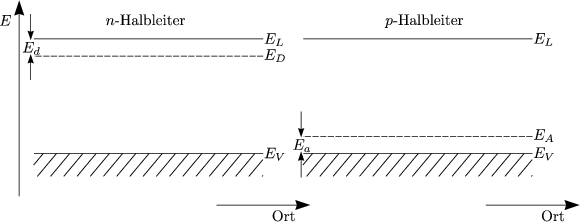
\includegraphics[width=0.8\textwidth]{images/BS_neu.png}
    \caption{Abbildung der durch eine Dotierung veränderten Bandstruktur eines Halbleiters. Links ist die n-Dotierung und rechts 
    die p-Dotierung dargestellt \cite{BS_neu}.}
    \label{}
\end{figure} \noindent
Bei einem Metall liegt kein Bandlücke vor. Außerdem ist das Leitungsband bereits zum Teil gefüllt. Somit reichen
bereits beliebig kleine Feldstärken aus, damit Elektronen in einen höheren Zustand übergehen können. Sie können 
als frei angenommen werden. 
\newpage
\section{Aufbau}
In Abbildung \ref{fig:Aufbau} ist das Interferometer mit dem Laser dargestellt. Der Detektionspfad zur Messung der Interferenzstrahlung ist nicht aufgezeigt.
\begin{figure}
  \centering
  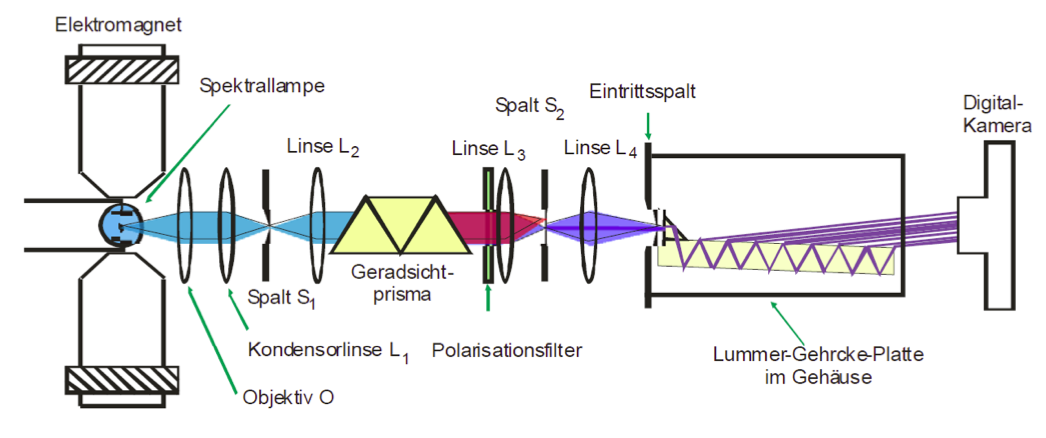
\includegraphics[width = .8\textwidth]{bilder/Aufbau.png}
  \caption{Aufbau des Sagnac-Interferometer ohne den Detektionspfad hinter dem PBSC (Punkt 10).}
  \label{fig:Aufbau}
\end{figure}
Als Strahlungsquelle des Sagnac-Interferometers dient ein \ce{HeNe}-Laser ($\lambda = \SI{632.99}{\nano\meter}$).
Der Laserstrahl wird zuerst durch zwei Spiegel auf einen Polarisationsfilter abgelenkt.
Mit dem Polarisationsfilter lässt sich aus dem linear polarisierten Laserstrahl eine Polarisationsrichtung auswählen.
Der Strahl trifft nach dem Polarisationsfilter auf den PBSC und wird dort nach seiner Polarisationsrichtung transmittiert (horizontale Polarisation), oder um \SI{90}{\degree} reflektiert (vertikale Polarisation).
Der weitere Aufbau ist geprägt durch 3 Spiegel, die mit dem PBSC ein Viereck bilden (vgl. Abbildung \ref{fig:Aufbau}).
Das vorher transmittierte Licht trifft somit an der Stelle auf den PBSC, an der das reflektierte Licht den PBSC verlassen hat und umgekehrt.
Somit werden sowohl transmittiertes und reflektiertes Lich nach ihrem Durchgang durch das Sagnac-Interferometer, wie zuvor, transmittiert und um \SI{90}{\degree} reflektiert.
\par\medskip
Weiterhin wird zur Erzeugung von Phasenverschiebungen eine Vorrichtung aus zwei Glasplättchen in den Strahlengang, zwischen Punkt 8 und 9, eingebaut.
Diese können, durch eine Drehscheibe, ihre Ausrichtung zum Strahlengang des Laserlichts verändern und so die Phasendifferenz beieinflussen.
Außerdem sind sie von ihrer Grundposition jeweils um einen festen Winkel gegen den Strahlengang gedreht.
\par\medskip
Für die Messung des Kontrastes des Interferometers unterscheidet sich der Aufbau von dem restlichen Versuchsteil.
Hinter dem PBSC wird im Detektionspfad ein weiterer Polarisationsfilter und hinter diesem eine Photodiode aufgebaut.
Dieser Polarisationsfilter sorgt dafür, dass nur die Polarisation einer bestimmten Richtung transmittiert werden und es so überhaupt zu Interferenzen kommt.
Um die benötigte Phasendifferenz für die Intensitäten $I_\text{min}$ und $I_\text{max.}$ zu erzeugen, wird der Strahlengang durch ein Verstellen des Spiegels M2 so auf den PBSC gelenkt, dass sich der Strahlengang örtlich aufteilt und auf die beiden Glasplättchen trifft.
Durch die Rotation dieser beiden Glasplättchen können die Intensitäten $I_\text{max.}$ und $I_\text{min.}$ für jeden Polarisationswinkel $\Theta$ des ersten Polarisationsfilters bestimmt werden und daraus der Kontrakt $K$ für diesen Polarisationswinkel bestimmt werden.
\par\medskip
Zur Messung des Brechungsindex der Glasplättchen wird im Detektionspfad statt dem Polarisationsfilters ein weiterer PBSC aufgebaut.
Sowohl das reflektierte Licht als auch das transmittierte Licht dieses PBSC trifft dann auf je eine Photodiode.
Aus der Differenzspannung der beiden Photodioden kann somit die Anzahl der $2\pi$ Phasenverschiebungen aus den Nulldulgängen bestimmt werden.
\par\smallskip
Der selbe Aufbau des Detektionspfads wird auch für die Messung der Brechungsindex für Luft in Abhängigkeit des Luftdrucks genutzt.
Die Glasplättchen werden aus den beiden Strahlen entfernt und dafür eine Druckkammer in einen der beiden Strahlen gestellt.
Der Druck in der Druckkammer kann durch eine Vakuumpumpe reduziert und über ein Ventil mit Luft geflutet werden.

\newpage
\section{Aufbau}
In Abbildung \ref{fig:schemAufbau} ist der schematische Versuchsaufbau dargestellt. Verwendet wird
eine Halogenlampe, deren Wellenlängenbereich größtenteils im infraroten Bereich liegt.
\begin{figure}[H]
    \centering
    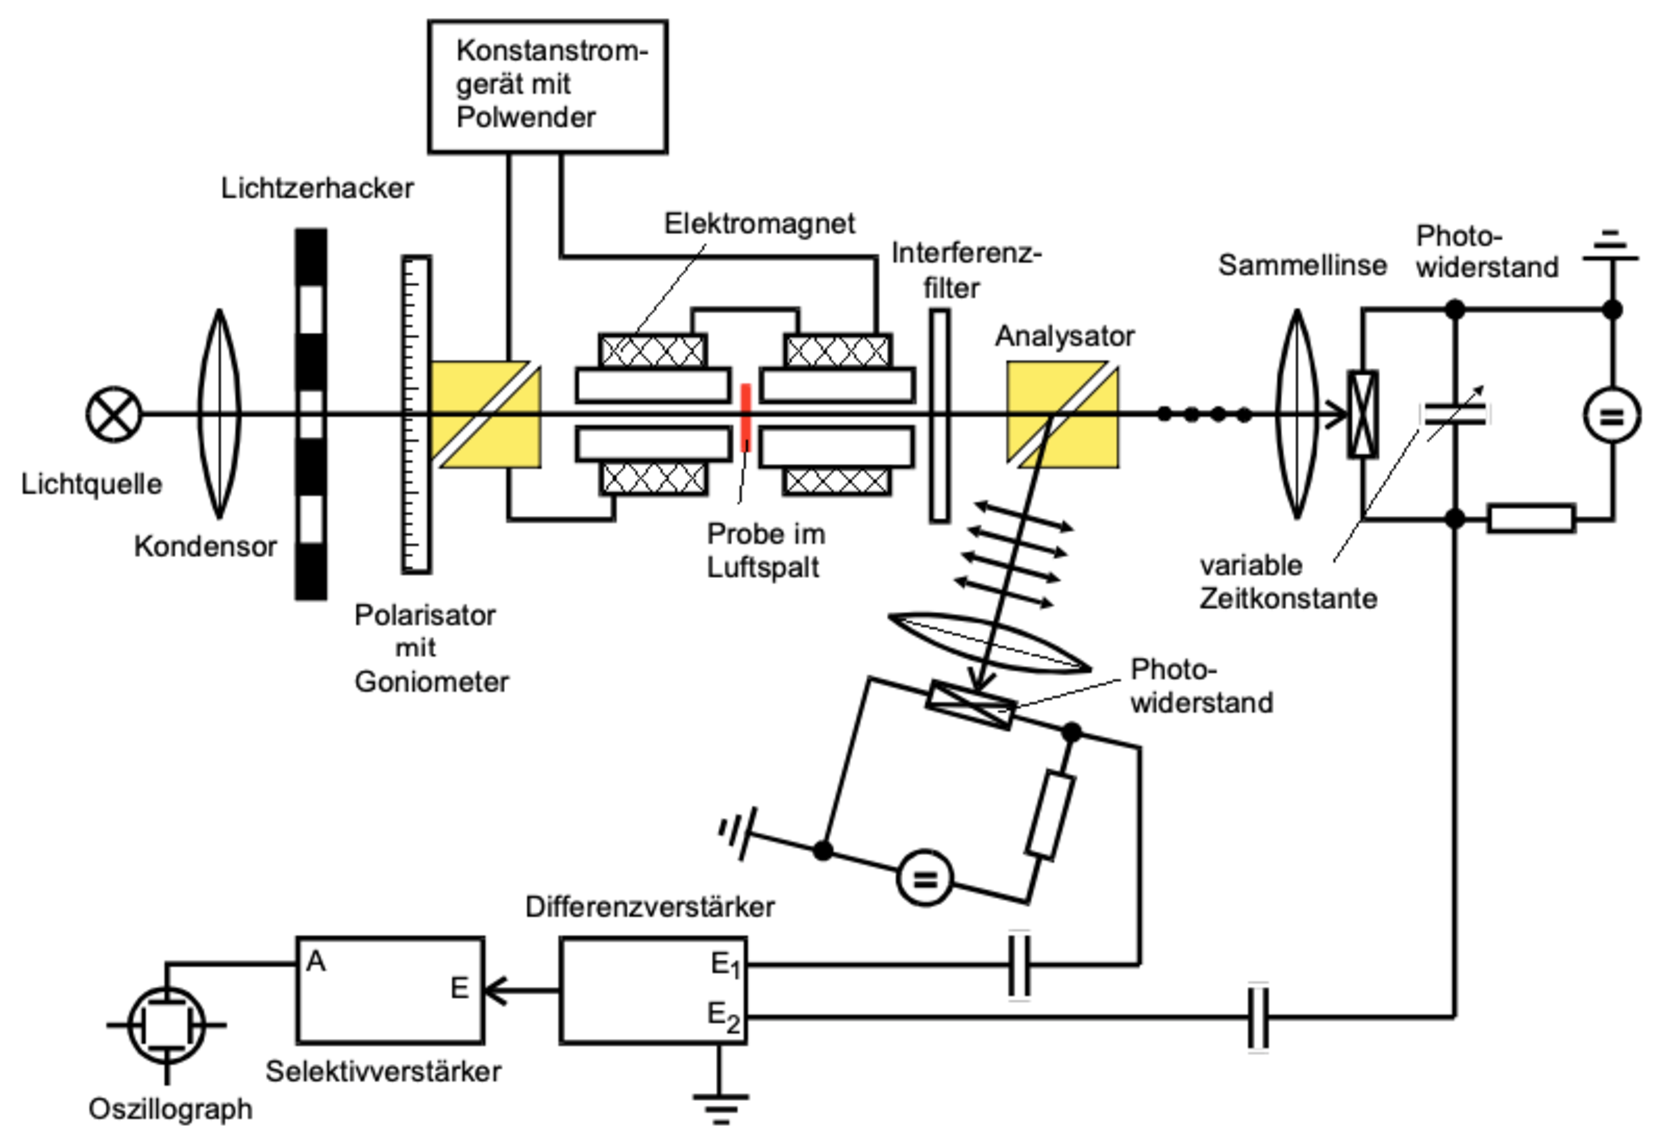
\includegraphics[width=0.8\textwidth]{images/SchemAufbau.pdf}
    \caption{Schematische Abbildung des verwendeten Versuchsaufbaus zur Bestimmung der effektiven
     Masse mithilfe des Faraday-Effekts \cite{anleitung}.}
    \label{fig:schemAufbau}
\end{figure} \noindent
Mithilfe einer Kondensorlinse wird das Licht der Halogenlampe parallelisiert bevor es den Lichtzerhacker passiert.
Daraufhin durchläft das Licht das erste Glan-Taylor-Prisma. Dieses sorgt dafür, dass auf die sich im
Elektromagneten befindliche Probe das notwendige linear polarisierte Licht trifft. 
Nachdem das Licht die Probe und die Elektromagneten durchdrungen hat, trifft es auf einen Interferenzfilter.
In diesem Versuch werden neun unterschiedliche Interferenzfilter im Bereich von $\SI{1.06}{\micro\meter}$ bis $\SI{2.65}{\micro\meter}$
verwendet. Durch das zweite verwendete Glan-Thompson-Prisma werden die Polarisationsanteile des 
eintreffenden Lichtes getrennt, sodass zwei Teilstrahlen entstehen. Die Intensitäten dieser werden
individuell mithilfe von Photowiderständen gemessen und in den Differenzverstärker eingespeist. Dieser 
berechnet wie der Name vermuten lässt, die Differenzen der beiden eintrefenden Signale. Dieses
Differenzsignal wird daraufhin durch den Selektivverstärker verstärkt und vom Oszilloskop visualisiert. 
Die Nutzung zweier Photowiderstände bietet eine hohe Genauigkeit. Da aufgrund der Differenzrechnung das
Finden des Minimums einfacher ist. Zusätzlich ist eine Messung mit dieser Methode nicht so anfällig
gegenüber Wellenlängen- oder Intensitätsschwankungen der Halogenlampe.
Wenn stattdessen nur eine Photodiode zum Einsatz kommt, muss ein Minimum im gemessenen Signal gefunden 
werden. Oftmals würden jedoch eine Vielzahl von Drehwinkeln einem solchen Kriterium entsprechen 
und die Aufnahme der Messwerte würde ungenauer. 

\section{Durchführung}
Bevor mit der eigentlichen Messung begonnen werden kann, muss eine Justage der Versuchsapperatur durchgenommen 
werden. Dafür wird überprüft, ob die durch das zweite Glan-Thompson-Prisma entstehenden Teilstrahlen auf
die lichtempfindlichen Flächen der Photowiderstände treffen. Dafür werden die Gehäuse von den Photowiderständen
entfernt und die Position des Glan-Thompson-Prismas angepasst. Ist eine gute Position der beiden 
Teilstrahlen gegeben, wird der Lichtzerhacker eingeschaltet und die Frequenz des Selektivverstärkers auf
die Frequenz des Lichtzerhackers eingestellt. Gewüscht ist ein maximales Signal, wenn das Signal eines 
Photowiderstandes direkt auf den Selektivverstärker gegeben wird. Ist dies der Fall wird der 
Gütefaktor auf 100 geregelt. Zur letzten Überprüfung der Justage werden eine Probe, sowie ein
Interferenzfilter eingesetzt und die Signale der Photowiderstände auf die beiden Eingänge des 
Differenzverstärkers gelegt. Beim Durchgehen eines großen Winkelbereichs am Polarisator sollte im Abstand von ca. 
$\SI{90}{\degree}$ periodisch ein minimales Signal zu beobachten sein. Ist dies nicht der Fall, sollte 
die Justage erneut vorgenommen werden. Ein besonderes Augenmerk sollte dabei auf dem Konstrast liegen. 
Idealerweise verschwindet einer der Teilstrahln, während der andere eine maximale Intensität aufweist. \\
\\
Nachdem die Justage erfolgreich abgeschlossen ist, wird mit der eigentlichen Messung begonnen. Zunächst 
wird die hochreine Galium-Arsenit Probe in den Versuchsaufbau eingefügt. Mithilfe des Oszilloskops 
wird der Polarisationswinkel gesucht bei dem sich das minimales Signal einstellt. Dieser wird notiert und
daraufhin das Magnetfeld umgepolt und der Vorgang wiederholt. Auf diese Weise wird die Probe im Zusammenspiel
mit den neun verschiedenen Interferenzfiltern untersucht. \\
Analog dazu werden zwei n-dotierte Galium-Arsenit Proben untersucht. Dabei handelt es sich bei Probe 1 
um eine $\SI{1.36}{\milli\meter}$ dicke Probe mit einer Ladungsträgerdichte von
$\SI{1.2e18}{\cubic\centi\meter}$. Die zweite Probe ist $\SI{1.296}{\milli\meter}$ dick und weist eine 
Ladungsträgerdichte von $\SI{2,8e18}{\cubic\centi\meter}$ auf. \\
Im letzten Schritt der Durchführung wird das vorherrschende Magnetfeld in der Nähe des im Elektromagneten 
vorhandenen Luftspaltes mithilfe einer Hallsonde ausgemessen und die Werte notiert.
\newpage
\section{Auswertung}

Alle Ausgleichsrechnungen werden mit dem Paket \texttt{scipy.optimize.curve\_fit}  aus \texttt{Python 3.7.3} durchgeführt.
Für Rechnungen mit fehlerbehafteten Größen wird das Paket \texttt{uncertainties} aus \texttt{Python 3.7.3} verwendet.\\

\subsection{Justage}
Zunächst wird eine Temperaturmessung und Justage durchgeführt. Mithilfe eines digitalen Thermometers wird die Temperatur
auf \SI{21.5}{\degreeCelsius} bestimmt. Nach dem Einstellen der in der Versuchsanleitung \cite{anleitung} aufgeführten Startwerte
werden diese solange variiert bis die gewünschten Signale zu sehen sind.
Die richtige Frequenz ist daran zu erkennen, dass das gemessene Signal keine Schwingungen mehr aufweist. Ist die richtige Frequenz
eingestellt wird die Phase variiert ist es das Ziel, dass sich das gesamte Signal ausschließlich im Realteil befindet.
Das bedeutet es wird versucht die Phase so zu verändern, dass eines der beiden angezeigten Signale möglichst verschwindet.
Beim Einstellen der Gradienten ist darauf zu achten, dass das FID-Signal möglichst lange zu erkennen ist.
Unter Berücksichtigung dieser Vorgehensweisen ergeben sich
\begin{align*}
  \text{Frequenz}&=\SI{21.72088}{\mega\hertz} \\
  \text{Phase} &= \SI{30}{\degree} \\
    x&=–1,7 \\
    y&=–5,1 \\
    z&=3,7 \\
    z^2 &=–2,4
\end{align*} \noindent
für die eingestellten Werte. \\
Die Bestimmung der Pulslängen für den $\SI{90}{\degree}$- und $\SI{180}{\degree}$-Puls ergibt
\begin{align*}
  \SI{180}{\degree} &= \SI{5.04}{\micro\second}\\
  \SI{90}{\degree}  &= \SI{2.52}{\micro\second}.
\end{align*} \noindent

\subsection{$T_1$-Messung}
Zur Bestimmung der $T_1$-Zeit wird die Magnetisierung für verschiedene Pulsabstände $\tau$ bestimmt.
Eine solche Messung ist beispielhaft in Abbildung \ref{fig:t1} dargestellt. Deutlich wird, dass eine vollständige Unterdrückung
des Imaginärteils, dargestellt durch den grünen Graphen, nicht gelungen ist. Außerdem sind zwei Ausschläge zu erkennen, wobei der
erste dem $\SI{180}{\degree}$-Puls zuzuordnen ist und der zweite dem $\SI{90}{\degree}$-Puls, der in diesem
Versuchsteil untersucht werden soll.
\begin{figure}[H]
  \centering
  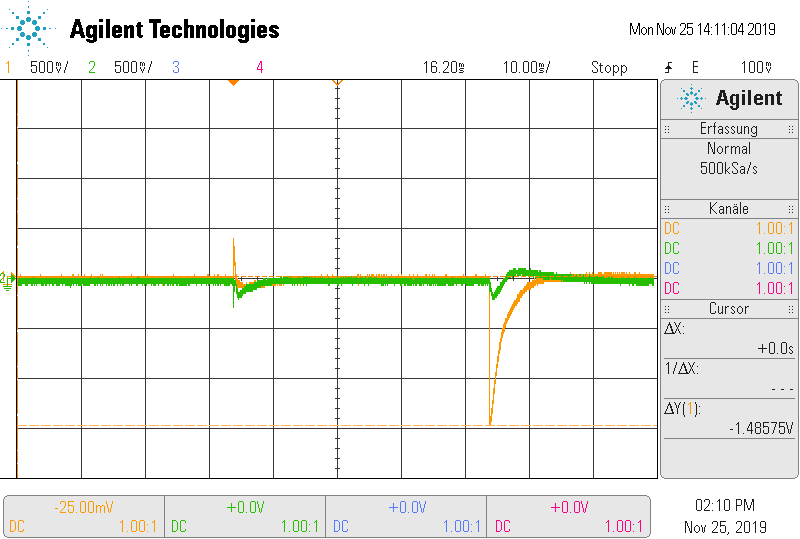
\includegraphics[width=0.8\textwidth]{../data/T1.png}
  \caption{Beispielhafte Darstellung einer Messung zur Bestimmung der $T_1$-Relaxationszeit. Untersucht wird der zweite zu
  erkennende Ausschlag, da er dem $\SI{90}{\degree}$-Puls zugeordnet ist. Beachtet wird dabei nur der Realteil des Signals,
  der durch den \textcolor{orange}{orangen} Graphen repräsentiert wird.}
  \label{fig:t1}
\end{figure} \noindent
Die bei der Messung mithilfe der Cursorfunktion bestimmten Signalstärken sind in Abbildung \ref{fig:t1_fit} gegen den
jeweiligen Pulsabstand $\tau$ zusammen mit einer Ausgleichskurve aufgetragen.
\begin{figure}[H]
  \centering
  \includegraphics[width=0.9\textwidth]{../Auswertung/t1_fit.pdf}
  \caption{Die aufgenommen Messwerte der Signalstärke in Abhängigkeit der Pulslänge $\tau$, sowie die
  zur Bestimmung der $T_1$-Zeit durchgeführte Ausgleichskurve. Für die x-Achse wird eine
  logarithmische Achse verwendet.}
  \label{fig:t1_fit}
\end{figure}
Durch die aufgenommenen Messwerte wird ein Ausgleichgraph der Form
\begin{equation*}
  M(\tau) = M_0 \cdot \exp(–\tau/T_1) + M_1
\end{equation*}
gelegt. Diese Regression liefert
\begin{align*}
  T_1 &= \SI{1.35(005)}{\second} \\
  M_0 &= \SI{3.00(005)}{\volt} \\
  M_1 &= \SI{-1.40(005)}{\volt}
\end{align*} \noindent
für die Relaxationszeit $T_1$, sowie die Magnetisierungsparameter $M_0$ und $M_1$.
Idealerweise stehen die Parameter $M_0$ und $M_1$ im Zusammenhang mit $M_0 = -2M_1$ \cite{anleitung}. Bei den durch die Regession bestimmten
Werten ergibt sich ein Verhätnis von
\begin{equation*}
  \frac{M_0}{M_1} = 2.22.
\end{equation*}
Das bedeutet, dass durch die durchgeführte Justage nicht die exakten Einstellungen vorgenommen worden sind. Dies lässt
sich zum Einen auch schon daran erkennen, dass sowohl Real- als auch Imaginärteil noch zu erkennen sind.

\subsection{$T_2$-Messung}
Im ersten Versuchsteil zur Bestimmung der $T_2$-Zeit wird der MG-Schalter auf \textit{on} gestellt. Somit
wird hier die Meiboom-Gill-Methode angewendet.
In Abbildung \ref{fig:t2} ist das aufgenommene Signal dargestellt. Es ist gut zu erkennen, das es den gewünschten Verlauf mit vielen Echosignalen zeigt.
\begin{figure}[H]
  \centering
  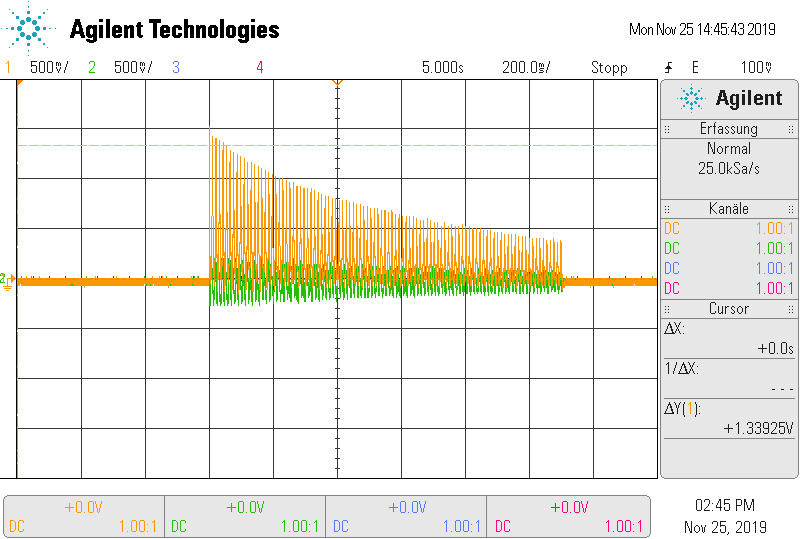
\includegraphics[width=0.8\textwidth]{../data/T2.png}
  \caption{Das aufgenommene Signal zeigt bei der Meiboom-Gill-Methode den gewünschten Verlauf. Die Signalstärke ist nach dem
  100. Maximum auf ca. $\frac{1}{3}$ der Maximalhöhe abgefallen. In \textcolor{orange}{orange} ist der untersuchte
  Realteil des Signals zu sehen.}
  \label{fig:t2}
\end{figure} \noindent
Zur Bestimmung der Relaxationszeit $T_2$, wird eine Ausgleichskurve der Form
\begin{equation*}
  M(t) = M_0 \cdot \exp(–t/T_2) + M_1
\end{equation*}
an die Einhüllende des oszilliereden Signals angepasst.
Dazu werdend die Maxima der Werte bestimmt und diese zur Berechnung des Ausgleichsgraphen verwendet.
Diese ist zusammen mit den Messwerten in Abbildung \ref{fig:T2_fit}
dargestellt.
\begin{figure}[H]
  \centering
  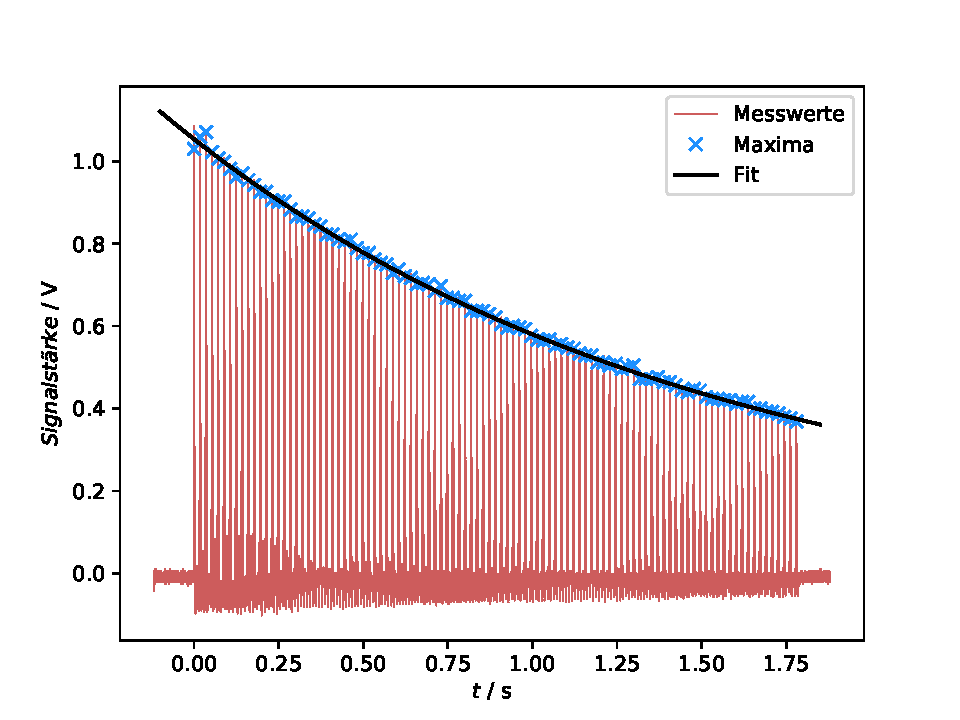
\includegraphics[width=0.9\textwidth]{../Auswertung/T2_fit.pdf}
  \caption{Die zur Bestimmung der $T_2$-Zeit durchgeführte Ausgleichsrechnung. In \textcolor{indianred}{rot} ist die Ausgleichskurve zu erkennen,
  die an die Einhüllende (\textcolor{dodgerblue}{blau}) des oszillierenden Signals (\textcolor{gray}{grau}) angepasst wird.}
  \label{fig:T2_fit}
\end{figure} \noindent
Die Regression liefert
\begin{align*}
  %M_0 &=  \SI{4791977.76(352863663)}{\milli\volt} \\
  %M_1 &=  \SI{188.18(5080)}{\milli\volt} \\
  T_2 &=  \SI{0.56(005)}{\second}
\end{align*}
für die gesuchte Spin-Spin-Realaxationszeit $T_2$. \\
Im Vergleich dazu ist in Abbidung \ref{fig:t2_off} das aufgenommene Signal für die Carr-Purcell-Methode zu sehen. Das heißt bei diesem
Messteil ist der MG-Schalter auf \textit{off} gestellt.
\begin{figure}[H]
  \centering
  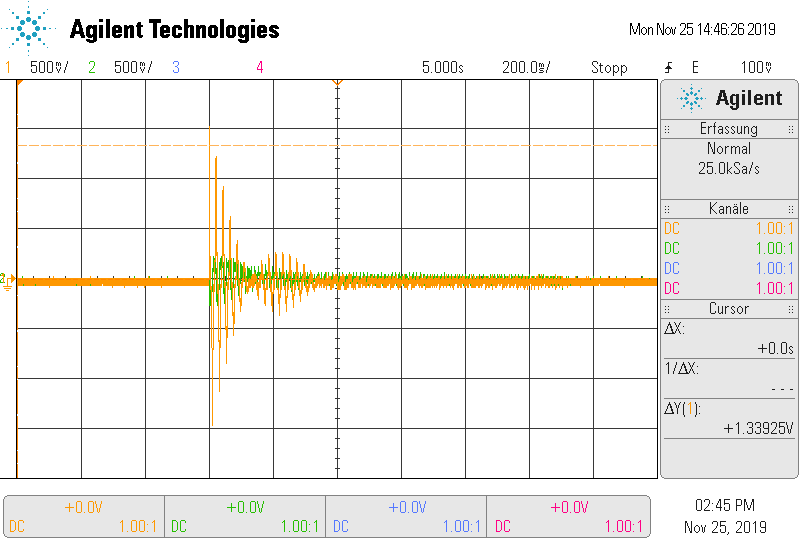
\includegraphics[width=0.8\textwidth]{../data/scope_76.png}
  \caption{Das aufgenommene Signal für die Carr-Purcell-Methode. Dabei ist deutlich zu erkennen, dass es durch die angelegten
  $\SI{180}{\degree}$-Pulse zum Wechsel zwischen Maxima im positiven und negativen Bereich kommt. Dabei repräsentiert der \textcolor{orange}{orangene} 
  Verlauf den Realteil des Signals und der \textcolor{green}{grüne} Veraluf den Imaginärteil.}
  \label{fig:t2_off}
\end{figure} \noindent
Es wird deutlich, dass im Gegensatz zu dem aufgenommenen Signal der Meiboom-Gill-Methode bei dieser Aufnahme die Maxima zwischen
dem positiven und negativen Bereich alternieren. Dies ist auf die geschalteten $\SI{180}{\degree}$-Pulse zurückzuführen.
Weiterhin nimmt das Signal deutlich schneller ab, als mit Meiboom-Gill-Methode, dies zeigt die Ungenauigkeit des \SI{180}{\degree}-Pulses.
Zur Verdeutlichung des typischen Verlaufs eines Spin-Echo Signals ist in Abbildung \ref{fig:N1} ein Signal dargestellt mit nur einem
geschalteten B-Puls.
\begin{figure}[H]
  \centering
  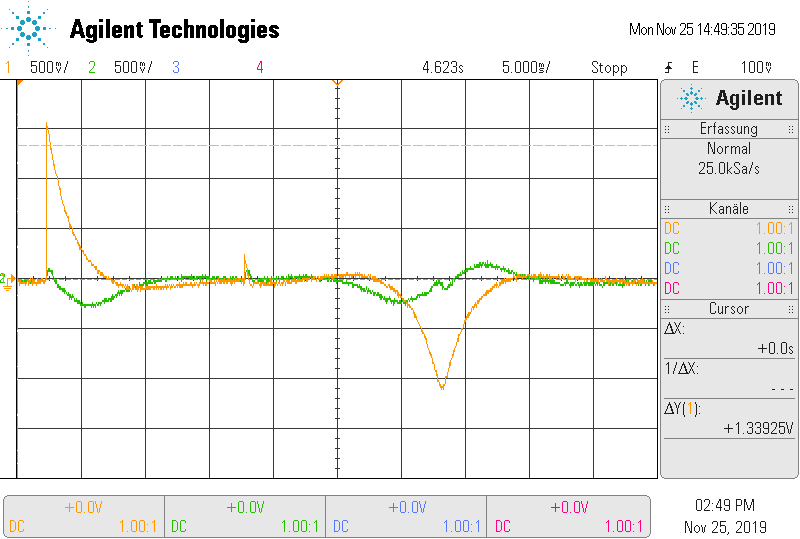
\includegraphics[width=0.8\textwidth]{../data/scope_77.png}
  \caption{Das aufgenommene Signal, wenn nur ein einziger B-Puls geschaltet ist. Zu Beginn des Signals ist der
  $\SI{90}{\degree}$-Puls zu erkennen. Nach dem $\SI{180}{\degree}$-Puls baut sich das Signal durch die Rephasierung
  wieder auf. Dabei repräsentiert der \textcolor{orange}{orangene} 
  Verlauf den Realteil des Signals und der \textcolor{green}{grüne} Veraluf den Imaginärteil.}
  \label{fig:N1}
\end{figure} \noindent
Zu erkennen ist zu Beginn des aufgenommenen Signals der $\SI{90}{\degree}$-Puls, der die Magnetisierung in die x-y-Ebene kippt.
Daraufhin kommt es zur Dephasierung der Spins mit der $T_2$-Zeit. Der $\SI{180}{\degree}$-Puls, der durch einen kleinen Ausschlag
zwischen dem Maximum und Minimum zu erkennen ist, sorgt für eine Rephasierung. Diese führt zu einem messbaren Signal, welches
jedoch aufgrund der Spin-Gitter-Wechselwirkung eine geringere Signalstärke aufweist.

\subsection{Diffusionsmessung}
In Abbildung \ref{fig:diff_fit} sind die gemessenen Echohöhen gegen den Pulsabstand $\tau$ auftragen.
Zusätzlich dazu wird eine Ausgleichskurve der Form
\begin{equation*}
  M(\tau) = M_0 \cdot \exp(–2\tau/T_2)\cdot \exp(–\tau^3/T_D) + M_1
\end{equation*}
mithilfe der Messwerte bestimmt. Dabei beschreibt $T_D$ die Diffusionszeit. Zur Bestimmung der gesuchten Parameter wird
die zuvor bestimmte $T_2$-Zeit verwendet.
\begin{figure}[H]
  \centering
  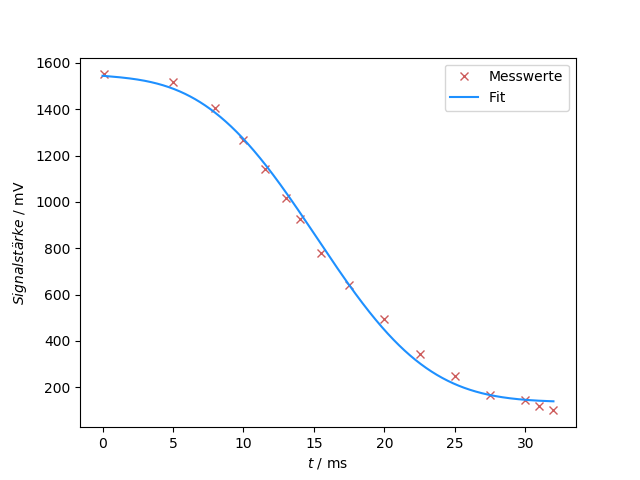
\includegraphics[width=0.8\textwidth]{../Auswertung/Diff_fit.png}
  \caption{Die gemessenen Echohöhen aufgetragen gegen den Pulsabstand $\tau$. Zur Bestimmung der Diffusionszeit $T_D$ wird eine
  Ausgleichskurve bestimmt.}
  \label{fig:diff_fit}
\end{figure} \noindent
Die Regression liefert
\begin{align*}
  M_0 &= \SI{1.41(002)}{\volt} \\
  M_1 &= \SI{0.14(002)}{\volt} \\
  T_D &= \SI{5.57(025)e-6}{\second}
\end{align*}
für die gesuchten Parameter.
Mithilfe des Zusammenhangs in Gleichung \eqref{eqn:TDiffusion}
kann die Diffusionskonstante bestimmt werden. Dabei beschreibt G den Gradienten des Magnetfelds $B_0$ , der mittels Fouriertransformation eines Echos
bestimmt wird. In Abbildung \ref{fig:echo_vorher} ist das verwendete Echo bei einem Pulsabstand von $\tau = \SI{0.0155}{\second}$ dargestellt. Wobei sowohl der Imaginär- als auch der Realteil
zu sehen sind.
\begin{figure}[H]
  \centering
  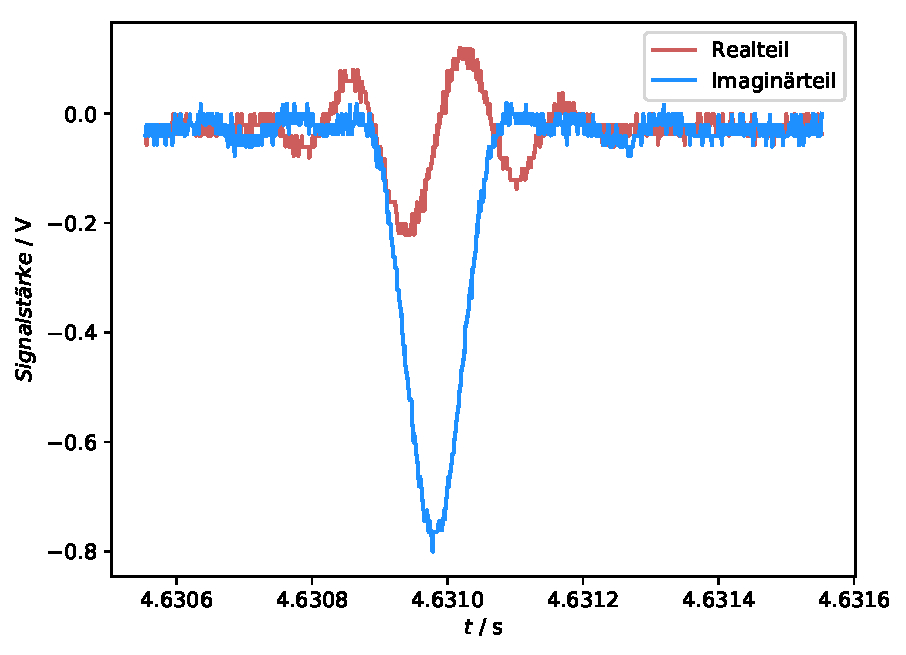
\includegraphics[width=0.9\textwidth]{../Auswertung/echo_vorher.pdf}
  \caption{Das zur Berechnung des Gradienten verwendete Echo bei einem Pulsabstand von $\tau = \SI{0.0155}{\second}$
  vor dem Abschneiden am Maximum und der durchgeführten
  Phasenkorrektur. In \textcolor{indianred}{rot} ist der Real- und in \textcolor{dodgerblue}{blau} der Imaginärteil des Signals dargestellt.}
  \label{fig:echo_vorher}
\end{figure} \noindent
Bevor eine Fouriertransformation durchgeführt werden kann, müssen die Messwerte des Signals so dargestellt werden, dass sie
beim Maximum des Realteils des Signals starten. Diese veränderte Darstellung des Signals ist zur Verdeutlichung des Vorgehens in
Abbildung \ref{fig:echo_ab} visualisiert.
\begin{figure}[H]
  \centering
  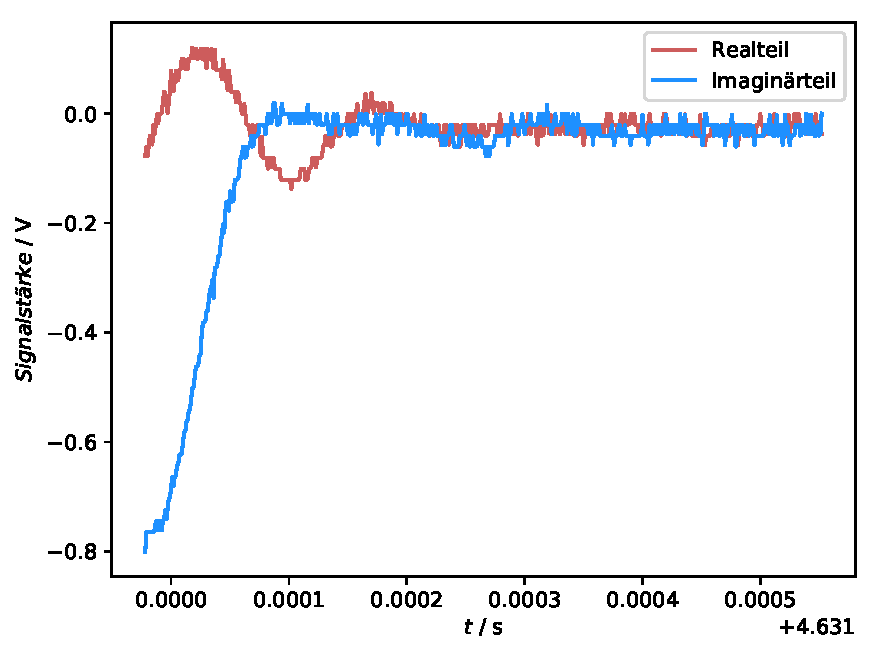
\includegraphics[width=0.9\textwidth]{../Auswertung/echo_abgeschnitten.pdf}
  \caption{Das zur Fouriertransformation vorbereitete Signal. Zu sehen sind sowohl der Realteil (\textcolor{indianred}{rot}) als auch der
  Imagainärteil (\textcolor{dodgerblue}{blau}) des Signals, beginnend beim Maximum des gemessenen Realteils.}
  \label{fig:echo_ab}
\end{figure} \noindent
In Abbildung \ref{fig:ft} ist das zu Abbildung \ref{fig:echo_ab} gehörige Frequenzspektrum abgebildet, das mithilfe der
Fouriertransformation bestimmt wird. Dieses Spektrum gibt die Verteilung der Larmorfrequenzen der Protonen wieder.
Aufgrund des geschalteten Gradienten unterscheidet diese sich abhängig vom Ort der Protonen.
\begin{figure}[H]
  \centering
  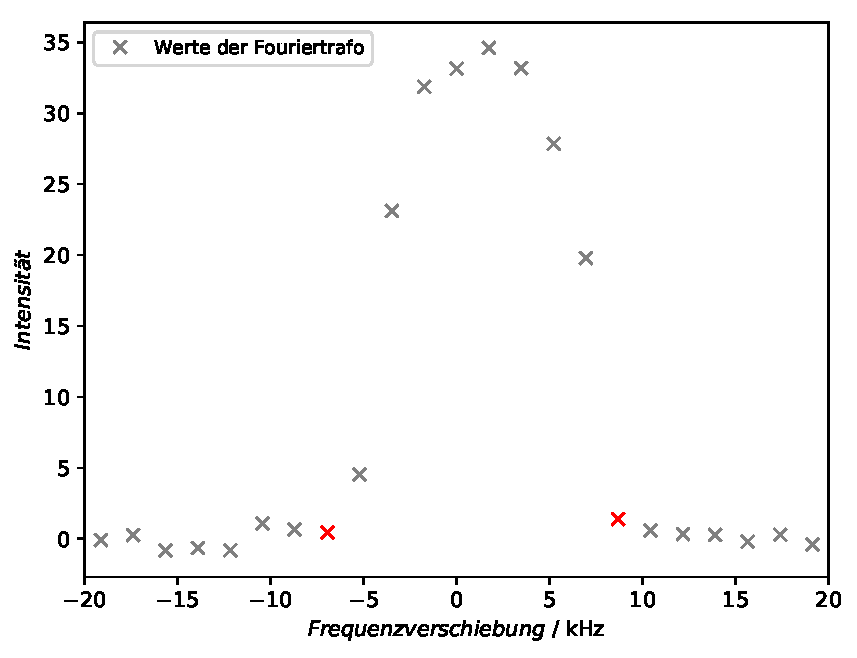
\includegraphics[width=0.9\textwidth]{../Auswertung/echo_ft.pdf}
  \caption{Das Ergebnis der auf das Echo angewendete Fouriertransformation. Mithilfe der Bestimmung der Breite der Frequenzverbreiterung
  ist es möglich den Gradienten und darüber die Diffusionskonstante zu berechnen.}
  \label{fig:ft}
\end{figure} \noindent
Die Frequenzbreite wird zwischen den beiden rot dargestellten Messwerten zu
\begin{align*}
  d_f = \SI{22.43}{\kilo\hertz}
\end{align*}
bestimmt.
Damit ist es über den Zusammenhang
\begin{align*}
  G = \frac{2\pi d_f}{\gamma d}
\end{align*}
möglich den vorliegenden Gradienten zu
\begin{align}
  G = \SI{0.125}{\tesla\per\meter}
\end{align}
zu bestimmen. Dabei wird mit $d = \SI{4.2}{\milli\meter}$ der Durchmesser des Probenröhrchens verwendet.
Mit dem bestimmten Grradienten und Gleichung \eqref{eqn:TDiffusion} kann die Diffusionskonstante zu
\begin{align}
  D = \SI{2.41(011)e-10}{\square\meter\per\second}
\end{align}
bestimmt werden.
Daraus ergibt sich mit einer Viskosität von $\eta \approx \SI{2.95}{\milli\pascal\second}$ \cite{viso} und einer
Temperatur von ca. $\SI{21.5}{\degreeCelsius}$
mithilfe von Formel \eqref{eqn:stokes}
\begin{align}
  r = \SI{3.04(014)}{\angstrom}
  \label{eqn:radius1}
\end{align}
für den Molekülradius des verwendeteten 1-Butanol. \\
Zum Vergleich wird der Molekülradius mithilfe des Molekulargewichtes und der Dichte berechnet. Dabei wird die Annahme getroffen,
dass die Moleküle in der vorliegenden Flüssigkeit eine hexagonal dichteste Kugelpackung bilden.
Da die Packungsdichte einer hexagonal dichtesten Kugelpackung mit
\begin{align*}
  \frac{\pi}{3\sqrt{2}} \approx \SI{74}{\percent}
\end{align*}
bekannt ist, ergibt sich für die Dichte
\begin{align*}
  \rho &= \frac{m_\text{ges}}{V_\text{ges}} \\
       &= \frac{\pi m_\text{But}}{3\sqrt{2}V_\text{But}}\,.
\end{align*}
Unter der Annahme, dass die 1-Butanol-Moleküle kugelförmig sind und somit für ihr Volumen
\begin{align*}
  V_\text{But} = \frac{4}{3} \pi r^3
\end{align*}
gilt, ergibt sich für den gesuchten Molekülradius
\begin{align}
  r = \sqrt[3]{\frac{m_\text{But}}{4\sqrt{2}\rho}} \approx \SI{2.99}{\angstrom}\, .
  \label{eqn:radius2}
\end{align}
Dabei wird $m_\text{But}$ mithilfe einer Molaren Masse von $\SI{74.12}{\gram\per\mole}$ berechnet.
Die Dichte von 1-Butanol beträgt bei Raumtemperatur ca. $\SI{0.81}{\gram\per\cubic\meter}$ \cite{dichte}.

\newpage
\section{Diskussion}
Die in diesem Versuch ermittelten Relaxationszeiten für die untersuchte 1-Butanol-Probe sind
\begin{align*}
  T_1 &= \SI{1.35(005)}{\second} \\
  T_2 &= \SI{0.56(005)}{\second} \, .
\end{align*}
Für die $T_2$-Zeit und die Diffusionskonstante von Butanol konnten keine Literaturwerte gefunden werden, deshalb werden diese Werte im Folgenden mit denen von Wasser bzw. Pentanol verglichen.

Der theoretische Wert der $T_1$-Zeit entspricht $T_1 = \SI{2.66}{\second}$ \cite{T1}, somit weicht der experimentell bestimmte Wert um $\SI{49.2}{\percent}$ von dem Literaturwert ab.
Ein Grund hierfür könnte eine nicht exakte Einstellung der Pulslängen für den \SI{90}{\degree}- und den \SI{180}{\degree}-Puls sein. Aufgrund eines zu kleinen Umklappens erscheinen die Signale kleiner und es wird eine kürzere $T_1$-Zeit bestimmt.

Die $T_2$-Zeit von Wasser beträgt nach \cite{chang} $T_2 = \SI{1.53(9)}{\second}$ und ist damit in etwa drei mal so lang wie die experimentell bestimmte $T_2$-Zeit von Butanol.
Durch die höhere Anzahl an Protonen in Butanol ist dort auch die Spin-Spin-Wechselwirkung größer und es kommt zu einer kleineren $T_2$ Zeit.

Allgemein lässt sich sagen, dass die sowohl die longitudinale als auch die transversale Relaxationszeit stark temperaturabhängig
sind. Eine Temperaturmessung bei jeder durchgeführten Messung hätte gegebenfalls zu genaueren Ergebnissen geführt,
als eine einmalige Temperaturmessung nach der Durchführung aller Versuchsteile.
Zudem war eine genaue Temperaturmessung innerhalb der Probenkammer nicht möglich, sodass die gemessene Raumtemperatur als
Temperatur angenommen worden ist. \\
\\
Im Allgemein liegt eine Fehlerquelle in der vorgenommenen Justage. Wie bei der Bestimmung der $T_1$-Zeit auffällt liegt
das gewünschte Verhältnis zwischen $M_0$ und $M_1$ nicht vor, sondern weicht um $\SI{11}{\percent}$ ab.
Es ist nicht gelungen den Imaginärteil des Signal vollständig auszulöschen, sodass lediglich der Realteil zurückbleibt.
Dies kann zu einer Verfälschung der Messergebnisse führen. \\


Die Bestimmung der Diffusionskonstante ergibt
\begin{align*}
  D = \SI{2.41(011)e-10}{\square\meter\per\second}\,.
\end{align*}
Dieser weicht stark von dem Literaturwert von Wasser $D_\text{W} = \SI{2.57(2)e-9}{\square\meter\per\second}$ \cite{wang} ab.
Ein Vergleich mit dem, von der Struktur her ähnlichen, 1-Pentanol liegt allerdings näher, da Pentanol nur eine Kohlenstoffverbindung mehr als 1-Butanol aufweist.
Die Diffusionskonstante von 1-Pentanol beträgt \SI{2.86e-10}{\square\meter\per\second} bei \SI{25}{\degreeCelsius} \cite{Holz} und liegt damit in der gleichen Größenordung wie die ermittelte Diffusionskonstante von 1-Butanol.


Die bei der Bestimmung des Molekülradius erzielten Ergebnisse aus \eqref{eqn:radius1} und \eqref{eqn:radius2} weichen lediglich um $\SI{1.7}{\percent}$ voneinander ab.
Obwohl bei der Rechnung die Annahmen eines ideal kugelförmigen Moleküls und einer hexagonal dichtesten Kugelpackung
angenommen worden sind, liegen die Ergebnisse dicht beieinander.

\newpage
\printbibliography
\end{document}
